
\section{The sideways force and the random kicks}\label{ch07:alphaprime}

\subsection*{A prediction that failed, and a coefficient that is zero}

The registered prediction for $\alpha'$ was the Iordanskii one: a weighted regression of $\hat\alpha'$ on $\rho_n/\rho$ over the temperatures, $T=0$ included, with a slope in $[0.6,1.4]$; ``no transverse force'' was a $2\sigma$ upper bound on the slope below $0.3$. In the frame of the simulation box the values are
\emph{negative}: $\hat\alpha'=-0.0100\pm0.0015,\ -0.0154\pm0.0029,\ -0.0093\pm0.0106$ at the three bases of \cref{ch07:tab-alpha} ($+0.0014$ at $T=0$), a slope of $-0.31\pm0.05$, $18\sigma$ from the Iordanskii window. The registered prediction is \textbf{refuted}, and the rule returns ``no transverse force''.
A negative $\alpha'$ has no theory behind it, though, and it was not left there: two kinematic facts about a compressible pair on a torus, both measured at $T=0$, explain most of it.

First, a single pair carries field momentum $2\pi nd$, which in a periodic box is a mean superfluid velocity $u=2\pi d/L^2$ of the whole fluid, absent from the periodic point-vortex velocity: in a $T=0$ sweep of single pairs the ratio of measured to torus point-vortex speed rises in the box frame from @@PS_D6@@ at $d=6$ to @@PS_D16@@ at $d=16$ (the saved file \texttt{pair\_speed\_T0.json}; the programme's note quotes $1.06$ and $1.49$), and in the fluid frame, which the ledger reports and which is not re-derived here, the pair moves at the point-vortex speed to
$+1\%$ at $d=6$ and $+0.4\%$ for $d\ge8$ (CLAIM-082). For two antiparallel pairs $|u|\le2\times10^{-3}$ and the pairs move in opposite directions, so the correction is below $0.0002$: decisive for single pairs only. Second, a pair of finite size is a solitary wave of the compressible field, whose speed departs from the point-vortex one (the Jones--Roberts correction) by $+3$--$4\%$ at $d=3$--$4$,
$+1\%$ at $d=6$ and $+0.4\%$ for $d\ge8$. Subtracting this baseline at the pair sizes the fits use gives $\alpha'=-0.0060\pm0.0015,\ -0.0112\pm0.0031,\ -0.0055\pm0.0106$ (CLAIM-082), with an uncertainty of the same order from the mapping between fit weights and pair sizes: \textbf{$\alpha'$ is zero within about $1\%$}, and the Iordanskii values $+2.7\%$, $+5.3\%$, $+9.4\%$ are excluded. The
``vortices move faster than the point-vortex velocity'' of the first analysis was mostly the compressibility of tight pairs at $T=0$. This is a classical field at one cutoff; Shukla, Brachet and Pandit read a nonzero $\alpha'$, without error bars, in the truncated field~\cite{Shukla2014}, and with a different arrangement (antiparallel pairs, the $T=0$ baseline subtracted) we do not adjudicate. In the cutoff scan the box-frame $\hat\alpha'$ stays small and negative ($-0.017$ and
$-0.031$ at $k_c=2\pi/3$, $-0.005$ and $-0.004$ at $2\pi$): reported, unexplained.

\subsection*{The Einstein relation, as an identity}

Take the stochastic pair of \cref{ch07:model}: drift $\mathbf b=-2\alpha\,\mathbf d/|\mathbf d|^2$ on the separation and isotropic noise of diffusion constant $D=2\eta$ (the separation is the difference of two walkers). Its probability current for a density $p$ is $\mathbf J=\mathbf bp-D\nabla p$, and the equilibrium pair gas of the Coulomb-gas picture of the
transition~\cite{KosterlitzThouless1973} has $p\propto|\mathbf d|^{-K}$ with $K=2\pi\rho_s/T$.

\begin{leanbox}{EinsteinRelation}
\begin{lstlisting}[style=lean,basicstyle=\ttfamily\footnotesize]
@@LEAN{EinsteinRelation.lean}{27-28}@@

@@LEAN{EinsteinRelation.lean}{53-54}@@

@@LEAN{EinsteinRelation.lean}{66-67}@@

@@LEAN{EinsteinRelation.lean}{82-84}@@
\end{lstlisting}
\nopagebreak[4]\smallskip\noindent\textit{Statements only; the proofs are in the module.}
\end{leanbox}

The current vanishes at every separation if and only if $DK=2\alpha$; in vortex units the pair gas can be in detailed balance iff $\eta=\alpha T/(2\pi\rho)$, the relation of Mehdi et al.~\cite{Mehdi2023}. Three things the programme measures separately, the shrinking of a pair ($\alpha$), the random walk of its separation ($D$) and the stiffness ($K$), are tied by one identity, and
$R_E=\eta K/\alpha$ is $1$ exactly when the gas can be in equilibrium at that stiffness. The Lean statement adds not the physics, which is Einstein's of 1905, but the fact that the test statistic of the pre-registration is an identity of the model with the equilibrium it presupposes made explicit. That equilibrium is the hypothesis easy to read past: $|\mathbf d|^{-K}$ is an \emph{assumption} about the
state of the gas, and if the bath is not in equilibrium on the time scales sampled, $R_E\neq1$ is not a violation of the identity.

\begin{table}[!tb]\centering\small
\begin{tabular}{lccccc}
\toprule
$T/T_{\rm BKT}$ & $\gamma$ & $\eta$ & $K$ & $R_E$ & quoted\\
\midrule
@@EIN_ROWS@@
\bottomrule
\end{tabular}
\caption{The random kicks: the local exponent $\gamma$ of $\langle|e|^2\rangle-c_0$ against the lag (lags $20$--$400$), the diffusion constant $\eta$ from $\langle|e|^2\rangle=c_0+4\eta\tau$, the stiffness $K=2\pi\rho_s/T$, and $R_E=\eta K/\alpha$ with errors from $\eta$ alone ($\alpha$ held fixed). Rule E2 quotes $\eta$ only where $\gamma\in[0.8,1.2]$.}
\label{ch07:tab-kicks}
\end{table}

\Cref{ch07:tab-kicks} gives the measurement. The diffusion constant is read from the residuals of the regression, $\langle|e|^2\rangle(\tau)=c_0+4\eta\tau$, where the offset $c_0\approx0.2$--$1.2$ is the thermal jitter of the detected cores; at $T=0$ the residual is bounded at $0.005$. Rule E2, fixed before the analysis, quotes $\eta$ only where the local exponent on lags $20$--$400$ lies in $[0.8,1.2]$: that
admits one temperature of three, $T/T_{\rm BKT}=0.27$, where $R_E=@@RE2@@\pm0.7$; the two unquoted temperatures would give $@@RE1@@$ and $@@RE3@@$. The decision rule needed two admitted temperatures: \textbf{by the rule the Einstein relation is undecided}. Informally, and against the rule, the vortex diffuses at about $1.4$ to $3$ times the Einstein value, the excess falling with temperature: far from
the hundredfold surplus that Neely et al.\ measure in a trap with vibrating walls~\cite{Neely2024}, and not cleanly one. A closed field has no walls to blame. (At $T/T_{\rm BKT}=0.43$ the error of $\alpha$ is $67\%$ and would dominate the error of $R_E$.)

The sub-diffusive exponent at the lowest temperature, $0.71$, invites a reading as a regular island: bounded quasi-periodic motion about the point-vortex trajectory. Lean makes the logic of the test precise: a finite sum of cosines has increments bounded by twice the sum of its amplitudes, so every mean of squared increments is at most $4(\sum_k|a_k|)^2$ at any lag
(\Lthm{QuasiPeriodicBound}{msd_bound}), and \Lthm{QuasiPeriodicBound}{not_qp_of_msd_large} turns this into a refutation, whatever the frequencies and phases. The test is one-sided: growth refutes an island, a plateau never proves one. On lags $\ge100$ the exponents at the two cooler temperatures are $1.24$ and $1.10$, which is growth: the sub-diffusion is a short-lag regime of the jitter, not an island.

\section{The wind that was not}\label{ch07:wind}

The impulse $2\pi\rho_sd$ of a shrinking pair has to go somewhere. In a periodic box it goes into the phonons, which drift at $u=2\pi\rho_s(d_0-d)/(\rho_nL^2)$ along the pair, and friction, which acts on the velocity of the vortex relative to the normal fluid, is reduced: $\dot d=-2\alpha\,(1/d-u)$. This is the programme's hypothesis~W, and Lean has a theorem for it.

\begin{leanbox}{DissipativeVortexDynamics}
\begin{lstlisting}[style=lean,basicstyle=\ttfamily\footnotesize]
@@LEAN{DissipativeVortexDynamics.lean}{164-166}@@

@@LEAN{DissipativeVortexDynamics.lean}{229-232}@@
\end{lstlisting}
\nopagebreak[4]\smallskip\noindent\textit{The second statement is the module's negative control: the hypothesis $b\le d(0)$ cannot be dropped. The first is proved by a ``fence'' argument: a solution that went below $b$ would have to cross a level $b-\varepsilon$ with positive derivative, which the sign of the drive forbids.}
\end{leanbox}

With $a+b=d_0$ and $ab=1/w$, $w=2\pi\rho_s/(\rho_nL^2)$, the wind equation is $\dot d=-2\alpha w(d-a)(d-b)/d$, and when $wd_0^2>4$ it has two positive zeros: a pair starting at or above $b$ never falls below it. The library states the identification of the two forms in a comment; the book's new module makes it a theorem and states the stall for the equation as derived.

\begin{leanbox}[unbreakable]{Ch07\_DissipativePairs (new, not in the library)}
\begin{lstlisting}[style=lean,basicstyle=\ttfamily\footnotesize]
@@LEANBOOK{Ch07_DissipativePairs.lean}{138-140}@@
\end{lstlisting}
\nopagebreak[4]\smallskip\noindent\textit{\texttt{stallPoint w d0} is $[d_0+\sqrt{d_0^2-4/w}]/2$. The module also proves that the roots are real, ordered and positive with $a+b=d_0$, $ab=1/w$, that for $wd_0^2<4$ the right-hand side has no zero, and a negative control (the hypothesis on the starting point cannot be dropped); all with the three standard axioms.}
\end{leanbox}

For the box of this chapter ($L=64$, $\rho_n/\rho=@@RN64@@$) and $d_0=12$: $w=@@W64@@$, $wd_0^2=@@WD64@@>4$, and in the plane formula, which neglects the torus's image forces (with them the paper estimates nearer $9$), the stall point is $b=@@B64@@$ (the lower root is $a=@@A64@@$), approached exponentially at the linearised rate $\lambda=2\alpha w(b-a)/b=@@LAM64@@$, a time constant of about
$@@TAU64@@$ time units, with the measured $\alpha=0.0062$ (CVODE, \cref{ch07:fig-failures}a). A pair of $d_0=8$ should not stall ($wd_0^2=@@WD8@@<4$). Two single pairs of $d_0\approx12$ at $T=0.115$, run for $4000$ time units, do not annihilate, while the zero-impulse pairs of the same temperature shrink steadily: the four pairs of the two archived runs with $d_0=10$ go from @@G2_START@@ to @@G2_END@@ in $1500$ time units. In the archived data one
pair falls from $@@W1_D0@@$ to $@@W1_S1_MIN@@$ by $t\approx1800$ and then wanders between $@@W1_S1_LO@@$ and $@@W1_S1_HI@@$ (the late slope of $d^2$ is $4\%$ of the early one); the other falls to about $@@W1_S2_MIN@@$ and re-expands to $@@W1_S2_END@@$, back toward the stall point, so that by the letter of the registered criterion (late slope below $25\%$ of the early one) it does not stall, though in
substance it stops shrinking. The momentum of the modes with $|k|>1$ follows the impulse shed by the pair, with regression slopes $@@W3_S1@@$ and $@@W3_S2@@$ against the registered window $[0.5,1.2]$ ($@@W3_SM@@$ after the $25$-unit running means of \cref{ch07:fig-failures}b, which remove the attenuation caused by the jitter of the detected separation), and falls back when the pair re-expands. So far hypothesis~W is
supported; metastable counterflow states exist in the Fourier-truncated Gross--Pitaevskii equation~\cite{KrstulovicBrachet2011}, and here the counterflow would be generated by the pair itself.

\begin{figure}[!tb]\centering
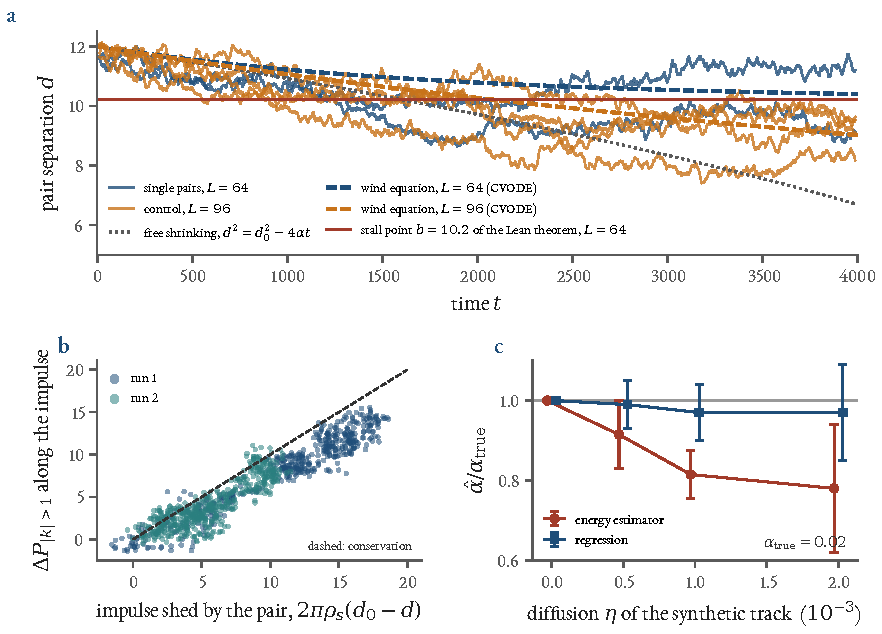
\includegraphics[width=\linewidth]{figures/ch07_failures.pdf}
\caption[Two theorems that were true and did not describe what they were applied to]{Two theorems that were true and did not describe what they were applied to. \textbf{a}~Separation of single pairs at $L=64$ (blue, two runs) and in the $L=96$ control (orange, four runs), $25$-unit running means, against the wind equation integrated with CVODE with the measured $\alpha=0.0062$ and no free parameter (thick dashed), free shrinking (dotted)
and the stall point $b$ of the Lean theorem (red). \textbf{b}~The wind seen directly: momentum of the phonon band $|k|>1$ projected on the initial impulse against the impulse shed by the pair, for the two $L=64$ runs; dashed, conservation of momentum between the pair and the phonons. \textbf{c}~The energy estimator of $\alpha$ on synthetic tracks of known $\alpha=0.02$ against the
diffusion $\eta$ of the track: exact at $\eta=0$ (the theorem), biased low when $\eta>0$; the regression estimator is not.}
\label{ch07:fig-failures}
\end{figure}

Then the control that the programme had registered as decisive was run. In an $L=96$ box at the same temperature ($\rho_n/\rho=@@RN96@@$) the same pair has $wd_0^2=@@WD96@@<4$: the equation has no zero (\Lthm{DissipativePairs}{wind_no_zero}), the box criterion $\rho_nL^2/(2\pi\rho_s)=@@C96@@$ exceeds $d_0^2/4=36$, and no stall is predicted. A pair that keeps shrinking supports the mechanism; a pair that stalls near the $L=64$
separation refutes it. With a tie-break of two further runs written in advance, the four runs ended at $d=9.3,\ 9.6,\ 8.3,\ 9.5$ (wind equation: $8.0$--$8.9$; free shrinking: $5.3$--$6.5$), and the late shrinking rate was $0$, $10$ and $37\%$ of the early one in runs 2--4, where the mechanism predicted about $50\%$. Only one of four meets the no-stall criterion, and the rule (at most one: refuted) gives the verdict:
\textbf{W2 is refuted; the pairs stall at $L=96$ as at $L=64$, the stall is not the box's, and the explanation by the phonon wind of a closed box is withdrawn.} The parameter-free wind curve of \cref{ch07:fig-failures}a shows that a drift of the normal component is \emph{consistent} with the data (all six pairs end within @@WV_MIN@@--@@WV_MAX@@ of the curve of their box, and @@WF_MIN@@ to @@WF_MAX@@ above free shrinking); consistent is not causal. The observation is kept (a reproducible, bath-driven stall
of a single pair at low temperature, with a $1/f^{0.5}$ separation spectrum), the explanation is not, and the graded test that could separate a residual wind from the real cause, a stall map in $L$, $d_0$ and $T$, is registered and has not been run. Every friction measurement on a single pair in a closed box at low temperature is affected, which is why the production runs use the zero-impulse geometry.

This is a clean example of what a proof assistant does and does not do. Lean certified the \emph{implication}: if the pair obeys the wind equation it cannot fall below $b$, and for $L=96$ the equation has no zero. The experiment tested the \emph{premise}, that the equation describes the pair, and refuted it. Nothing in the kernel could have said so.

\section{An estimator that was exact, and was not}\label{ch07:bias}

A second implementation is an instrument. The registered estimators were ported to Rust (crate \texttt{qf-pgpe}, module \texttt{transport}), first for speed, and the port agrees with the Python code on real tracks to $@@XCHK_RELDIFF@@$ (\cref{ch07:field}). Run on the registered synthetic gate G0 (known $\alpha=0.02$, $\alpha'=0.10$, $\eta=2\times10^{-3}$, eight tracks of $2000$ time units) over \emph{many seeds}, it showed what the single seed of
the gate had not.

With no diffusion the energy estimator returns the true value, exactly. With diffusion it is low, by @@BIAS_PCT@@ at $\eta=5\times10^{-4}$, $10^{-3}$, $2\times10^{-3}$, while the regression estimator is low by only @@BIAS_REG_PCT@@ (\cref{ch07:fig-failures}c). The means over @@BIAS_SEEDS@@ seeds of eight tracks each are @@BIAS_AE@@ for the energy estimator and @@BIAS_AR@@ for the regression estimator, for a true $\alpha=0.02$ and no detection noise (Rust example \texttt{g0\_scan --eta-scan} of \texttt{qf-pgpe}, run for this chapter); the ledger records the bias as independent of the detection noise (CLAIM-098). The gate's criterion (energy estimator within $15\%$) passes on $2$ of $12$ seeds (CLAIM-098); the registered gate had
passed on one lucky seed. In the real arms the regression estimator exceeds the energy one by $5$ to $21\%$, in exactly this direction.

Why did the theorem not warn us? Because it is not about this. Its hypothesis is \texttt{hr}: the path has a derivative at every instant and obeys the flow (\Lthm{DissipativeVortexDynamics}{energy_dissipation}). A diffusing vortex has no derivative; the identity belongs to the \emph{deterministic} model, and the data are not a path of that model. The cause of the bias is not proven (the programme's note suspects that the stochastic part of $H(t)$ is
correlated with the cumulative regressor $\int2S\,dt$, which depends on the same noisy path); what is proven is that the identity applies where its hypothesis holds, and there it is exact ($\alpha_{\rm energy}=0.0200$ at $\eta=0$). This is LL-15 applied to the programme's own tool: a conclusion travels with its preconditions or not at all. No registered verdict changes (they compare arms with the same estimator), but the absolute $\alpha$ of \cref{ch07:tab-alpha}
are low by about $5$--$20\%$ ($0.0062$, $0.014$, $0.02$ become $@@E060_AR@@$, $@@E070_AR@@$, $@@E080_AR@@$ with the regression estimator, \cref{ch07:tab-alpha}), the temperature law reads $0.060\,T$ rather than $0.054\,T$, and the gate's energy criterion is not a reliable known answer; the regression criterion is.

\section{What this chapter establishes, and what it does not}\label{ch07:honest}

\begin{honestbox}
\textbf{Proved in Lean (standard axioms only; checked on 2026-10-09).} The energy identity for any flow of the form~\eqref{ch07:eq-flow}; for the plane dipole, the law $|\mathbf d|^2=|\mathbf d_0|^2-4\alpha t$ and the centre velocity $(1-\alpha')/|\mathbf d|$, and, in the book's new module, the law $+4\alpha t$ of the same-sign pair; the zero-current characterisation $DK=2\alpha$; the kinetic identity for $\alpha/(\rho_n/\rho)$; the stall of the wind equation and, new, its stall at the root $b$; the bound on quasi-periodic mean-square displacements (\cref{ch07:lean,ch07:law,ch07:alphaprime,ch07:wind}). These are statements about \emph{models}, elementary and not new (the new theorems are in \texttt{book/lean/}, not in the library), and none is a statement of Godfrin's papers.

\textbf{Simulated, in a classical projected field (one box, $mg=1$, cutoffs $2\pi/3$, $\pi$, $2\pi$, $T<0.45\,T_{\rm BKT}$).} $\alpha=0.0062(4)$, $0.014(2)$, $0.02(1)$ at $T/T_{\rm BKT}=0.14$, $0.27$, $0.43$ by two estimators, the energy one low by $5$--$20\%$; $\alpha\simeq0.054\,T$ (energy) or $0.060\,T$ (regression) over three cutoffs; $\alpha'=0$ within about $1\%$ once the $T=0$ kinematics of a compressible pair on a torus are
accounted for; the diffusion $1.4$--$3$ times the Einstein value where it can be read; a bath-driven stall of a single pair; one fresh run of $1500$ time units, one seed, inside the scatter of single runs. CVODE reproduces the exact pair laws to $3\times10^{-8}$ (dipole) and $10^{-5}$ (rotating pair).

\textbf{Analogy only, not established.} Anything about helium, atomic gases, or the fluid whose excitations Godfrin measured: the classical-field bath is not a Bose bath (\cref{ch07:law}), the temperature of the field is a parameter of the model, and $\sigma_{\rm tr}(k)$ of a vortex has not been measured here. The Einstein relation is undecided by the registered rule.

\textbf{Failed, withdrawn or corrected.} The first known-answer gate passed on a defective imprint and is withdrawn (CLAIM-075). The reading $\alpha\propto\rho_n$ with a vortex-owned coefficient and the ``geometric core size'' $1.4\xi$ are withdrawn: the coefficient depends on the cutoff, and the registered predictions of FL2 and of the Born law failed. The registered Iordanskii-like prediction for $\alpha'$ is refuted at $18\sigma$. The phonon-wind mechanism is
refuted by the $L=96$ control while its Lean theorem stays true. The energy estimator is biased low by the diffusion, which no theorem was about. The temperature law was formulated after the data of five arms were read and is confirmed, by the registered window, on a sixth arm whose error is larger than was assumed.
\end{honestbox}

\section{Exercises}

\paragraph{Exercise 1.} Show that two vortices of the \emph{same} sign obey $|\mathbf d|^2=|\mathbf d_0|^2+4\alpha t$ and rotate with angular velocity $2(1-\alpha')/|\mathbf d|^2$ about their fixed centre, and find how long a pair with $d_0=4\xi$ and $\alpha=0.02$ takes to double its separation. Then reproduce panel~b of \cref{ch07:fig-dipole}: the listing of \cref{ch07:cvode} needs only a new right-hand side, for two vortices of the same sign.
\emph{Hint.} With $\mathbf d=\mathbf p_1-\mathbf p_2$ the velocities induced at the two vortices are $\pm\hat{\mathbf z}\times\mathbf d/|\mathbf d|^2$; the radial component of $\dot{\mathbf d}$ is $2\alpha/d$, so $d\,\dot d=2\alpha$; the answer to the first question is $3d_0^2/(4\alpha)=600$.

\paragraph{Exercise 2.} Generate synthetic dipole tracks with the Langevin generator of the repository (\texttt{exploration/pgpe/transport\_estimators.py}, function \texttt{langevin}) for $\alpha=0.02$ and $\eta=0$, then $\eta=10^{-3}$, and apply the energy and the regression estimators through \texttt{qf\_pgpe.analyse\_tracks}. Explain, from the hypotheses of \Lthm{DissipativeVortexDynamics}{energy_dissipation}, why the first case must be exact and why
the second need not be. \emph{Hint.} Look at \texttt{hr}: what regularity does a Brownian path have? Expect $\alpha_{\rm energy}\approx0.016$ at $\eta=10^{-3}$ over eight tracks of $2000$ time units.

\paragraph{Exercise 3.} (LL-15.) For $\varepsilon_k=\sqrt{k^2+k^4/4}$ at $T=0.115$ compute $n_{\rm RJ}/n_{\rm Bose}$, with $n_{\rm RJ}=T/\varepsilon_k$ and $n_{\rm Bose}=1/(e^{\varepsilon_k/T}-1)$, at $k=0.2,\,1,\,\pi$. Then compute the fraction of the equipartition Landau sum $\tfrac12L^{-2}\sum_kk^2T/\varepsilon_k^2$ carried by modes with $\varepsilon<T$, on the $3208$ modes of the disk $|k|\le\pi$,
$L=64$. Which statements of \cref{ch07:law} depend on the equipartition occupation, and which would survive in a Bose bath? \emph{Hint.} The first part is three lines of code; the second is a fraction of a per cent.

\section{Notes and further reading}

The programme's two papers on the subject are \cite{Callens2026a}, on friction, the transverse coefficient, the diffusion and the stall of a single pair (Zenodo, version~2.2, October 2026, \texttt{doi:10.5281/\allowbreak zenodo.23262143}), and \cite{Callens2026b}, on the cutoff scan and the temperature law (\texttt{doi:10.5281/\allowbreak zenodo.23262132}); the engine is in \cite{Callens2026sw}, the Lean library in \cite{Callens2026lib}. The static half of the first paper, the box-scale pair, equilibration and the polarisability
of the pair gas, bears on the Kosterlitz--Thouless side of \cref{ch06} and is not treated here. For mutual friction in helium start with Donnelly's book~\cite{Donnelly1991} and the review of Sergeev~\cite{Sergeev2023}; for measurements in atomic gases, \cite{Moon2015} and \cite{Neely2024}, and, in a Fermi superfluid, where the friction and the vortex Hall angle were measured, \cite{Grani2025}; for the diffusion, \cite{Mehdi2023}, and for the stochastic point-vortex model as used
for helium films, \cite{AHNS1980}; for the transverse force, \cite{ThoulessAoNiu1996}, \cite{Iordanskii1964} and \cite{Sonin1997}. The point-vortex flow on the torus is in \cite{WeissMcWilliams1991}, and the integrability of few-vortex flows in the survey~\cite{ModinViviani2021}.
\widowpenalty=\chsevenwp\relax\clubpenalty=\chsevencp\relax
\flushbottom
